%Functional Requirements
\section{Functional Requirements}

Requirements are ordered by importance.

\begin{itemize}
\item{F1: Communication Library}\newline
The Android should use the Communication Library to connect wirelessly 
to an Arduino module and establish two way communication.

\item{F2: Social Library}\newline
Android applications should be able to retrieve social data from any 
supported social network through the use of the Social Library. General 
concepts applicable in any social network such as Person, Group, Message, etc.
should be extracted and devised into a model interface that is easy for the application
developer to use.

\item{F3: Wireless connectivity}\newline
Since the product will target a user-base with no technical background,
the customer required all connections between devices to be wireless,
so that connecting the User Interface to the Android mobile will be
as easy as possible for the end-users. For this reason, the technical
details of the connection should be hidden to the end-user so that
the product can be easily operated.

\item{F4: Prototype}\newline
To show that the concept of Tangible User Interfaces for Android applications
(including social networks) using Arduino is not only possible, but
also a feasible market product, the customer is interested in a working
prototype. Develop three prototypes, one more complex prototype showcasing the 
functionality of both the Communication Library and Social Library. The other
two prototypes should be much simpler in complexity and their purpose is just to
prove that the libraries can be successfully used for different prototypes.

\item{F5: Support Android platform 2.2}\newline
The library should be compatible with Android API version 2.2 and later. This is to
ensure that any application built with our library is compatible with as many Android
versions as possible. The specific version to be supported was set by the customer.
\end{itemize}


%Non functional Requirements
\section{Non-functional Requirements}

\begin{itemize}
\item{NF1: Flexible software architecture}\newline
The software that will be developed for this project will serve as
a proof-of-concept and possibily as a starting point for other research
projects. For this reason a flexible, modular software architecture
is an important requirement for our customer. The code shall be developed
in independent, thus reusable modules so that adding new functionality
will be fairly easy for new developers.

\item{NF2: Software licenses}\newline
The customer made clear that the software developed needs to be released
under a permissive, Apache compatible software license. This implies
that pre-existing software that will eventually be adopted and incorporated
in the project must have a compatible license.

\item{NF3: API Documentation and Javadoc}\newline
Since the product is going to be further developed by other people and is
mainly designed for easier application development then proper research and usage
documentation is important. Proper documentation or tutorials should describe how
the end-user can easily use the libraries without any technical knowledge of how
the library works.

\item{NF4: Target platforms}\newline
The product has to target the Android platform and Arduino.
This will place restrictions on the software and on the programming languages that will be adopted.
\end{itemize}

\newpage
\section{Use cases}
\todo{
	review.
}
Use Case:
We have two actors we are working with. One is the developer creating the application using our framework.
The other one is the end user with the final product. We are not directly working with the end user as an actor,
but we still want to make our framework so it is simple for developer to have a product with an easy connection to the arduino board.

Our focus on the actor developer is centered around the software he create. We do not know, and we don't need to
know what product he is making. We will work on two parts he can to implement in his software. It will be the setup and
transfer protocol to arduino and Intents to send and recive updates from social services.

For the end user, we want the setup to connect his phone to the developer to be as easy as possible. The focus will be on
simplified connection to arduino board, and easy connection to social services from application.

\todo{
	outdated?
}
\begin{figure}[hb!]
\centering 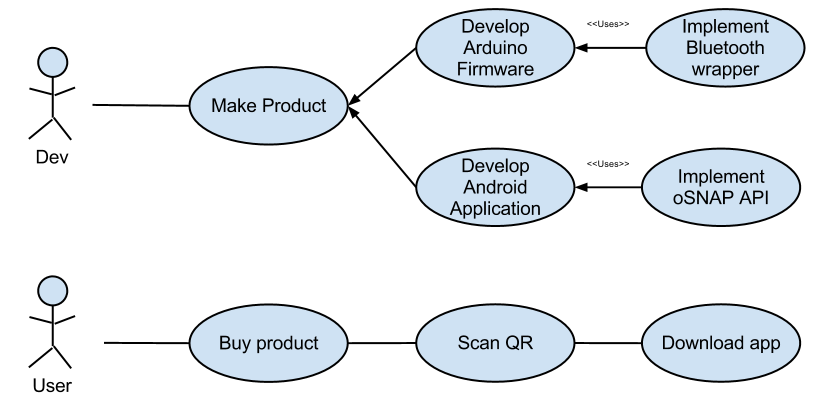
\includegraphics[scale=0.50]{img/use-cases.png}
\caption{Use cases}
\label{fig:architecture-usecases}
\end{figure}

First scenario.

\begin{figure}[hb!]
\centering 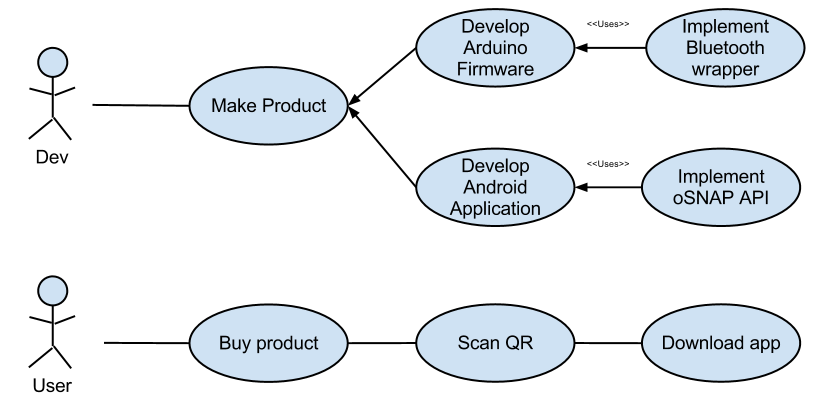
\includegraphics[scale=0.50]{img/use-cases.png}
\caption{First use case}
\label{fig:req-usecase1}
\end{figure}

Revised scenario.

\begin{figure}[hb!]
\centering 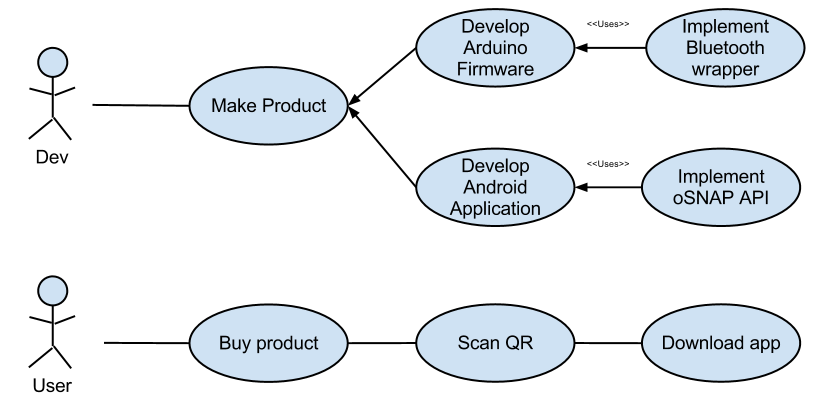
\includegraphics[scale=0.50]{img/use-cases.png}
\caption{Revised use case}
\label{fig:req-usecase2}
\end{figure}